\documentclass{sigchi}

% Use this command to override the default ACM copyright statement (e.g. for preprints). 
% Consult the conference website for the camera-ready copyright statement.
\toappear{
	Submitted for review.
}

% Arabic page numbers for submission. 
% Remove this line to eliminate page numbers for the camera ready copy
\pagenumbering{arabic}


% Load basic packages
\usepackage{balance}  % to better equalize the last page
\usepackage{graphics} % for EPS, load graphicx instead
\usepackage{times}    % comment if you want LaTeX's default font
\usepackage{url}      % llt: nicely formatted URLs



% llt: Define a global style for URLs, rather that the default one
\makeatletter
\def\url@leostyle{%
  \@ifundefined{selectfont}{\def\UrlFont{\sf}}{\def\UrlFont{\small\bf\ttfamily}}}
\makeatother
\urlstyle{leo}


% To make various LaTeX processors do the right thing with page size.
\def\pprw{8.5in}
\def\pprh{11in}
\special{papersize=\pprw,\pprh}
\setlength{\paperwidth}{\pprw}
\setlength{\paperheight}{\pprh}
\setlength{\pdfpagewidth}{\pprw}
\setlength{\pdfpageheight}{\pprh}


%graphics
\usepackage{tikz}

\usetikzlibrary{arrows,snakes,shapes}

\definecolor{darkred}{RGB}{127, 0, 0}
\definecolor{darkgreen}{RGB}{0, 127, 0}
\definecolor{lightgray}{RGB}{191, 191, 191}
\tikzstyle{processstep}=[draw,text width=3.5cm,text centered,minimum width=4cm,minimum height=1cm]
\tikzstyle{orientedarc}=[->,>=latex]
\tikzstyle{arc}=[<->,>=latex]
\tikzstyle{arclabel}=[midway,scale=0.7]
\tikzstyle{arclabelred}=[midway,darkred,scale=0.7]
\tikzstyle{arclabelgreen}=[midway,darkgreen,scale=0.7]

\tikzstyle{justleft}=[shift={(-0.5cm,0cm)}]
\tikzstyle{justright}=[shift={(0.5cm,0cm)}]
\tikzstyle{justtop}=[shift={(0cm,0.5cm)}]
\tikzstyle{justdown}=[shift={(0cm,-0.5cm)}]

\tikzstyle{architectureelement}=[draw,text width=1.7cm,text centered,minimum width=1.8cm,minimum height=2cm]
\tikzstyle{architecturelabel}=[text centered,text width=3cm]

\tikzstyle{breakline}=[snake=snake,segment length=1.8cm,segment amplitude=0.2cm]

\newenvironment{packed_enum}{
\begin{enumerate}
  \setlength{\itemsep}{1pt}
  \setlength{\parskip}{0pt}
  \setlength{\parsep}{0pt}
}{\end{enumerate}}


\newenvironment{packed_itemize}{
\begin{itemize}
  \setlength{\itemsep}{1pt}
  \setlength{\parskip}{0pt}
  %\setlength{\parsep}{0pt}
}{\end{itemize}}


% Make sure hyperref comes last of your loaded packages, 
% to give it a fighting chance of not being over-written, 
% since its job is to redefine many LaTeX commands.
\usepackage[pdftex]{hyperref}
\hypersetup{
pdftitle={SIGCHI Conference Proceedings Format},
pdfauthor={LaTeX},
pdfkeywords={SIGCHI, proceedings, archival format},
bookmarksnumbered,
pdfstartview={FitH},
colorlinks,
citecolor=black,
filecolor=black,
linkcolor=black,
urlcolor=black,
breaklinks=true,
}


% create a shortcut to typeset table headings
\newcommand\tabhead[1]{\small\textbf{#1}}


% End of preamble. Here it comes the document.
\begin{document}

\title{A formal language for next generation cockpits user interfaces specification}


\numberofauthors{3}
\author{
  \alignauthor Vincent Lecrubier\\
    \affaddr{ONERA/DTIM}\\
    \affaddr{Toulouse}\\
    \email{vincent.lecrubier@onera.fr}
  \alignauthor Bruno d'Ausbourg\\
    \affaddr{ONERA/DTIM}\\
    \affaddr{Toulouse}\\
    \email{ausbourg@onera.fr}
  \alignauthor Yamine A\"it-Ameur\\
    \affaddr{ENSEEIHT}\\
    \affaddr{Toulouse}\\
    \email{yamine@enseeiht.fr}
}


\maketitle

\begin{abstract}
  User interfaces take an important role in commercial success of past and future aircraft programs. They have a direct influence on flight safety, crew members opinion of the aircraft and the efficiency of aircraft operations. 
As computing power and complexity of systems increase, user interfaces must become more and more effective in order to allow human operators to deal with this complexity. The goal of this project is to develop a formal language which will enhance the development process,verification and validation of these user interfaces.
\end{abstract}

\keywords{
	Human Machine Interface; User Interface; Design; Specification; Verification; Validation; Formal Language.
}

\category{H.5.2.}{User Interfaces}{Evaluation/methodology}

\terms{
Design; Human Factors; Languages; Reliability; Security; Verification.
}

%====================================================================================================================================
% SECTION
%====================================================================================================================================
\section{ORIGIN AND UNDERLYING PRINCIPLES}
%What is the origin of the framework and what are its underlying principles?
  
Critical  embedded  UIs   (\emph{user  interfaces})  conception  is  a
discipline  which  lies at  the  limits  of  two software  engineering
domains:   embedded   software    development   and   user   interface
development. As a consequence,  critical embedded user interfaces must
comply with  a set  of conflicting constraints  coming from  these two
different domains.

While  embedded software  makes robustness  a priority,  UIs  must be
flexible  and  configurable.   While  embedded  systems  have  limited
ressources,   UIs   must   be   complete   and   integrate   lots   of
functionalities.   While   critical   software  have   strong   timing
constraints, UIs  must be user friendly  and let the  user interact at
his  own pace.  While critical  systems are  often real-time,  UIs are
mostly event-driven.

This  set  of conflicting  constraints  is  a  strong limitation  for
critical  UIs, and  makes  their development  particularly costly  and
time-consuming.

The apparition  of model-based development  has been a big  leap ahead
for non-critical UI  development, allowing for more complex  UIs to be
designed in a  quicker and cheaper way. However,  critical UIs did not
really  profit  yet  from  this   new  fresh  air.  They  indeed  lack
development  methodologies and  tools which  would be  compatible with
safety requirements while allowing quick and efficient development.

A good critical  UIs development process should take  into account the
methods   and  tools   in  use   for  both   of  these   domains  (see
Fig.~\ref{fig:domains}).

This project  tends to  make a constructive  use of formal  methods in
critical UIs development.  As so, it relies on  previous works on this
subject.  Many works  were already  performed on  formal  modelling of
software aspects of UIs by suggesting two main approaches. 

The first one is based on proof systems where a model of the system is
described by  sets of variables,  sets of operations, sets  of events,
timing properties and  invariants. Operations must preserve invariants
and  properties. To  ensure the  correctness of  these specifications,
proof obligations are generated and must be proved. So, for example, Z
and  VDM  were  used  to  define  atomic  structures  of  interactions
(\cite{Duke-Harrison93a},\cite{Duke-Harrison93b}) and  HOL (High Order
Logic Theorem  Prover) was used to check  user interface specification
(\cite{Bumbulis96}).  B  system was also  used for the  an incremental
specification   design   of   interactive  systems   (\cite{yamine98},
\cite{yamine04}).

%-----------------------------------------------------------   Figure   -----------------------------------------------------------
\newcommand{\Ca}{(0,0) ++(135:2)}
\newcommand{\Cb}{(0,0) ++(45:2)}
\begin{figure}
\centering
\resizebox{\linewidth}{!}{
\begin{tikzpicture}
\begin{scope}
\clip \Cb circle (2);
\fill[lightgray] \Ca circle (2);
\end{scope}
\draw \Ca circle (2); % A
\draw \Ca ++(0,-2) node [below] {Critical systems} ;
\draw \Ca ++(180:1) node [scale=0.7] {Model checking} ;
\draw \Ca ++(135:1) node [scale=0.7] {B Method} ;
\draw \Ca ++(-135:1) node [scale=0.7] {Static code analysis} ;
\draw \Ca ++(90:1.4) node [scale=0.7] {Theorem proving} ;
\draw \Ca ++(-90:1.4) node [scale=0.7] {Petri nets} ;
\draw \Cb circle (2); % B
\draw \Cb ++(0,-2) node [below] {User interfaces} ;
\draw \Cb ++(0:1) node [scale=0.7] {Prototyping} ;
\draw \Cb ++(45:1) node [scale=0.7] {Usability analysis} ;
\draw \Cb ++(-45:1) node [scale=0.7] {Human factors} ;
\draw \Cb ++(90:1.4) node [scale=0.7] {Extensive testing} ;
\draw \Cb ++(-90:1.4) node [scale=0.7] {Look \& Feel design} ;
\draw (0,0) ++(45:1) ++(135:1) node [text centered, rotate=0, scale=0.7, text width=1.7cm] {\bf Critical UIs} ;
\end{tikzpicture}
}
\caption{Critical UIs : collision of two clashing domains}
\label{fig:domains}
\end{figure}

The second one  is based on the evaluation of  logical properties of a
system  on a  state transition  system. This  technique was  used, for
example, to  verify formally with  SMV some properties  of interactive
systems    (\cite{Campos97}).    Model    checking    was   used    in
(\cite{Palanque95},\cite{Navarre03}) where the user and the system are
modelled by object Petri nets (ICOs). In \cite{Rushby01}, Mur$\phi$ is
used for modelling  an autopilot system and a mental  model in order to
analyse  cockpit interfaces  and  to detect  some potential  problems.
Model checking was also coupled  with static analysis of program codes
in \cite{ausbourg98}  or \cite{Cortier2008} to extract  and abstract a
formal model of an interactive  system and to check various properties
on it modelling and analysis of human-automation  interaction has also
been demonstrated \cite{6083931}.

This project  aims at inverting the approach  in \cite{ausbourg98} or
\cite{Cortier2008}  by  defining  a  language  which  would  allow  to
formaly describe model the behaviour  of UIs.  The model perimeter is
the \emph{dialog controller} and  \emph{Logical interaction} of the UI
Arch Model from \cite{Bass91}. The model will be using abstractions to
perform model checking on the high level behaviour of UIs.

%====================================================================================================================================
% SECTION
%====================================================================================================================================
\section{MODELLED RELATIONSHIPS}
%What relationships are captured in the framework’s models?

%-----------------------------------------------------------   Figure   -----------------------------------------------------------
\begin{figure*}
\centering
\resizebox{17cm}{!}{
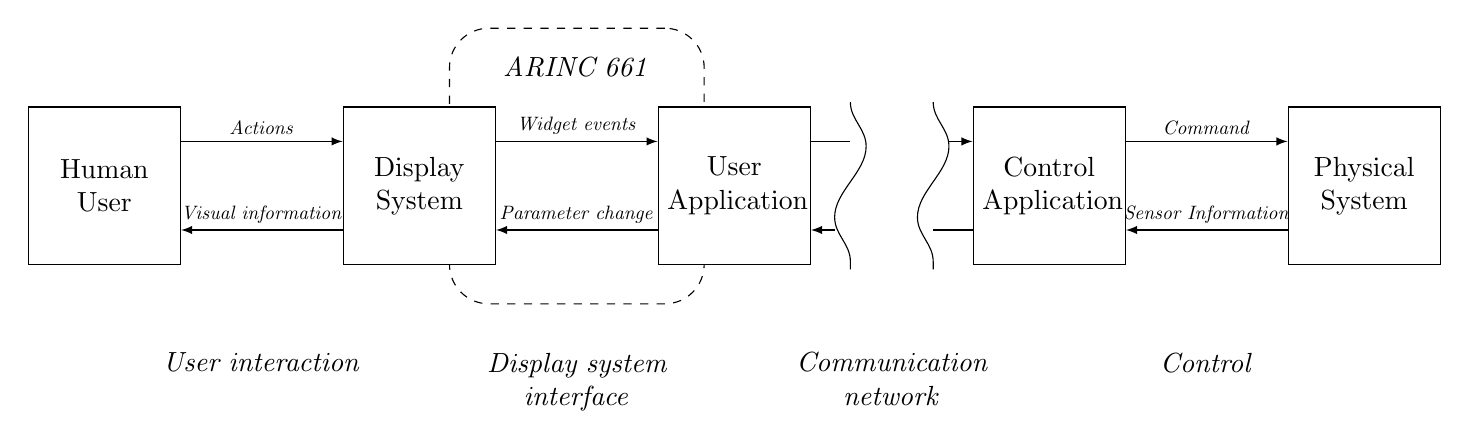
\begin{tikzpicture}
\tikzstyle{architectureelement}=[draw,text width=1.7cm,text centered,minimum width=1.8cm,minimum height=2cm,fill=white]
\tikzstyle{architecturelabel}=[text centered,text width=3cm]
\tikzstyle{breakline}=[snake=snake,segment length=1.8cm,segment amplitude=0.2cm]

\node[draw,text width=3cm,text centered,minimum width=3cm, minimum height=3.5cm,dashed,rounded corners = 0.5cm]
 (SARINCFRAME) at (6cm,0.25cm) {};
\node[text width=3cm,text centered,minimum width=3cm,minimum height=1cm]
 (SARINC) at ([shift=({0cm,-0.5cm})]SARINCFRAME.north) {\textit{ARINC 661}};


\node[architectureelement] (S1) at (0cm,0cm) {Human \\ User};
\node[architectureelement] (S2) at (4cm,0cm) {Display \\ System};
\node[architectureelement] (S3) at (8cm,0cm) {User \\ Application};
\node[architectureelement] (S4) at (12cm,0cm) {Control \\ Application};
\node[architectureelement] (S5) at (16cm,0cm) {Physical \\ System};

\node[architecturelabel,below] (L1) at (2cm,-2cm) {\textit{User interaction}};
\node[architecturelabel,below] (L2) at (6cm,-2cm) {\textit{Display system \\ interface}};
\node[architecturelabel,below] (L3) at (10cm,-2cm) {\textit{Communication network}};
\node[architecturelabel,below] (L4) at (14cm,-2cm) {\textit{Control}};

\coordinate[justright] (S3E1) at (S3.30);
\coordinate[justright] (S3E2) at (S3.-30);
\coordinate[shift={(0.3cm,0cm)}] (S3E2b) at (S3.-30);
\coordinate[justtop] (S3E3) at (S3E1);
\coordinate[justdown] (S3E4) at (S3E2);
\coordinate[justleft] (S4W1) at (S4.150);
\coordinate[shift={(-0.3cm,0cm)}] (S4W1b) at (S4.150);
\coordinate[justleft] (S4W2) at (S4.-150);
\coordinate[justtop] (S4W3) at (S4W1);
\coordinate[justdown] (S4W4) at (S4W2);

\draw[orientedarc] (S1.30) -- (S2.150) node[arclabel, above]{\textit{Actions}};
\draw[orientedarc] (S2.-150) -- (S1.-30) node[arclabel, above]{\textit{Visual information}};

\draw[orientedarc] (S2.30) -- (S3.150) node[arclabel, above]{\textit{Widget events}};
\draw[orientedarc] (S3.-150) -- (S2.-30) node[arclabel, above]{\textit{Parameter change}};

\draw[] (S3.30) -- (S3E1) node[arclabel, above]{\textit{}};
\draw[orientedarc] (S4W1b) -- (S4.150) node[arclabel, above]{\textit{}};

\draw[]  (S4.-150) -- (S4W2) node[arclabel, above]{\textit{}};
\draw[orientedarc] (S3E2b) -- (S3.-30) node[arclabel, above]{\textit{}};

\draw[breakline] (S3E3) -- (S3E4) node[arclabel, above]{\textit{}};
\draw[breakline] (S4W3) -- (S4W4) node[arclabel, above]{\textit{}};

\draw[orientedarc] (S4.30) -- (S5.150) node[arclabel, above]{\textit{Command}};
\draw[orientedarc] (S5.-150) -- (S4.-30) node[arclabel, above]{\textit{Sensor Information}};


\end{tikzpicture}
}

\caption{Aircraft UIs architecture. The UA interacts with the CDS one one side, and with other aircraft applications on the other side.}
\label{fig:architecture}
\end{figure*}

The language goal is to model the UAs (\emph{user applications}) which are applications that comply with the ARINC 661 Specification.
ARINC 661 is the industry standard for Cockpit Display System Interfaces to User Systems \cite{ARINC661}.

This formal language would take into account aspects of both abstract UIs and embedded systems :
\begin{packed_itemize}
\item{UIs (structure, internal behaviour, human interaction, interface with systems)}
\item{Critical systems (resources footprint, timing constraints, reliability, integrity)}
\end{packed_itemize}

A typical model specified using this language would be a closed system, with a static structure, interacting with two types of abstract external objects (see Fig.~\ref{fig:architecture}):
\begin{packed_itemize}
\item{Display System (e.g. CDS (\emph{Cockpit Display System}))}
\item{Application (e.g. Other aircraft application)}
\end{packed_itemize}

The system would be specified by organizing abstract components in order to generate the desired behaviour.
The modelled system would then allow to generate different projections:
\begin{packed_itemize}
\item{Models to be checked}
\item{ARINC 661 compliant code}
\item{Test cases and scenarios for validation}
\end{packed_itemize}

%====================================================================================================================================
% SECTION
%====================================================================================================================================
\section{PROBLEMS ADDRESSED}% For what problem is the framework intended or best suited?

  As of today, in order to pass qualification, UIs must undergo a massive, long test procedure, like many other pieces of embedded software. However, the fact that UIs interact directly with humans makes the conception process much heavier. Indeed, fully automatic generation of UIs still does not yield satisfactory results, and extensive automatic testing is not possible (see Fig.~\ref{fig:process1}).

  As a consequence, UIs have to be tested manually during the verification and validation phases. Since these tests happen at the end of the conception loop, errors found during manual tests can become excessively costly to correct, needing to get back in the conception loop.

%-----------------------------------------------------------   Figure   -----------------------------------------------------------
\begin{figure}
\centering
\resizebox{0.7\linewidth}{5cm}{
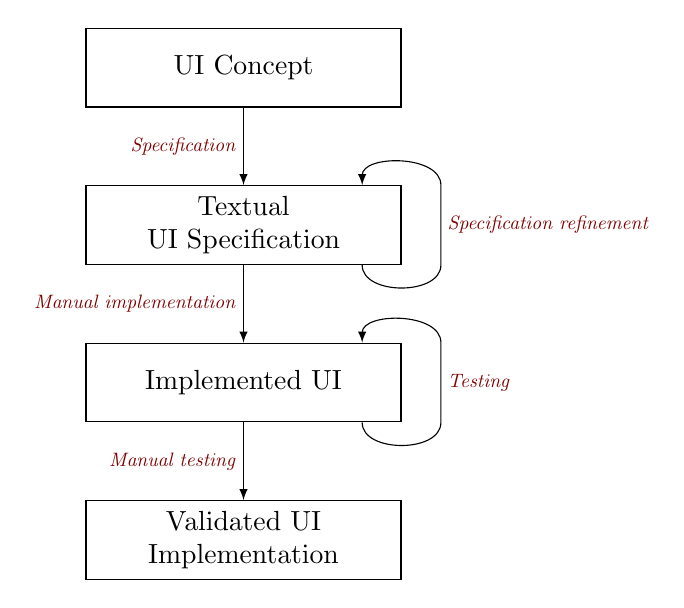
\begin{tikzpicture}

\node[processstep] (S1) at (0cm,6cm) {UI Concept};
\node[processstep] (S2) at (0cm,4cm) {Textual \\ UI Specification};
\node[processstep] (S3) at (0cm,2cm) {Implemented UI};
\node[processstep] (S4) at (0cm,0cm) {Validated UI \\ Implementation};

\coordinate[justright] (S2NORTHEAST1) at (S2.north east);
\coordinate[justright] (S2SOUTHEAST1) at (S2.south east);
\coordinate[justleft] (S2NORTHEAST2) at (S2.north east);
\coordinate[justleft] (S2SOUTHEAST2) at (S2.south east);

\coordinate[justright] (S3NORTHEAST1) at (S3.north east);
\coordinate[justright] (S3SOUTHEAST1) at (S3.south east);
\coordinate[justleft] (S3NORTHEAST2) at (S3.north east);
\coordinate[justleft] (S3SOUTHEAST2) at (S3.south east);

\draw[orientedarc] (S1) -- (S2) node[arclabelred, left]{\textit{Specification}};
\draw[orientedarc] (S2) -- (S3) node[arclabelred, left]{\textit{Manual implementation}};
\draw[orientedarc] (S3) -- (S4) node[arclabelred, left]{\textit{Manual testing}};
\draw[orientedarc] (S2SOUTHEAST2) to[bend right=90] (S2SOUTHEAST1) -- (S2NORTHEAST1) node[arclabelred, right]{\textit{Specification refinement}} to[bend right=90] (S2NORTHEAST2);
\draw[orientedarc] (S3SOUTHEAST2) to[bend right=90] (S3SOUTHEAST1) -- (S3NORTHEAST1) node[arclabelred, right]{\textit{Testing}} to[bend right=90] (S3NORTHEAST2);

\end{tikzpicture}
}

\caption{Classical UI conception process}
\label{fig:process1}
\end{figure}


%-----------------------------------------------------------   Figure   -----------------------------------------------------------
\begin{figure}
\centering

\resizebox{0.7\linewidth}{5cm}{

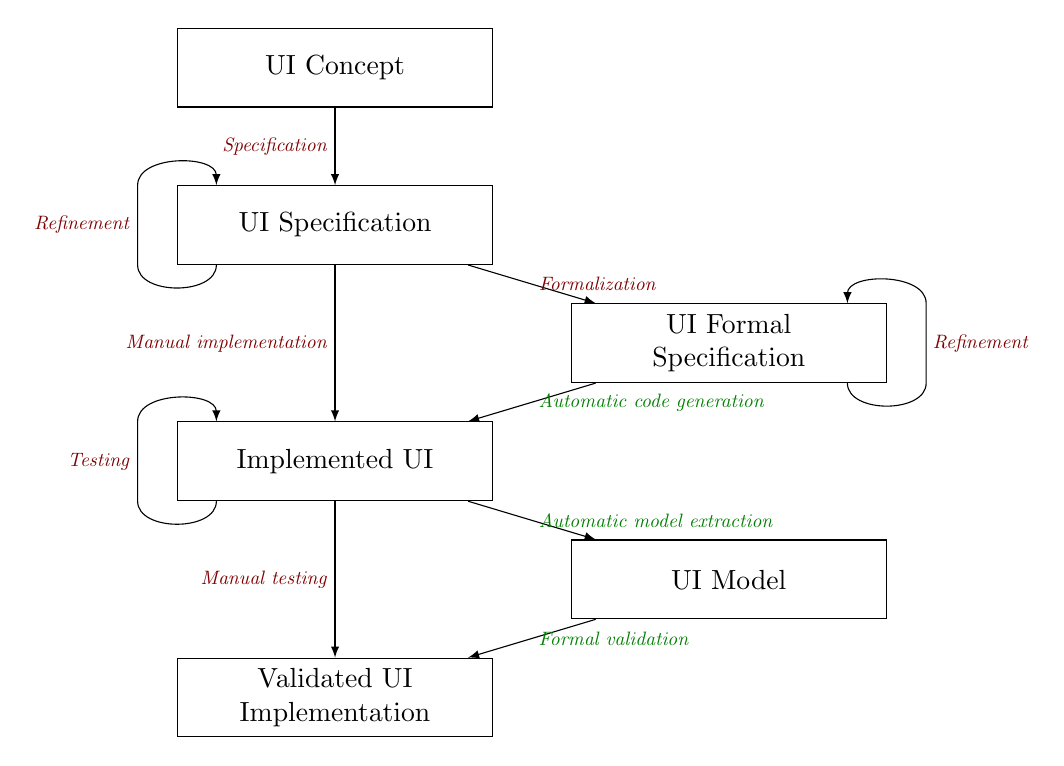
\begin{tikzpicture}

\node[processstep] (S1) at (0cm,8cm) {UI Concept};
\node[processstep] (S2) at (0cm,6cm) {UI Specification};
\node[processstep] (S3) at (0cm,3cm) {Implemented UI};
\node[processstep] (S4) at (0cm,0cm) {Validated UI \\ Implementation};
\node[processstep] (S5) at (5cm,4.5cm) {UI Formal \\ Specification};
\node[processstep] (S6) at (5cm,1.5cm) {UI Model};

\coordinate[justleft] (S2NORTHEAST1) at (S2.north west);
\coordinate[justleft] (S2SOUTHEAST1) at (S2.south west);
\coordinate[justright] (S2NORTHEAST2) at (S2.north west);
\coordinate[justright] (S2SOUTHEAST2) at (S2.south west);

\coordinate[justleft] (S3NORTHEAST1) at (S3.north west);
\coordinate[justleft] (S3SOUTHEAST1) at (S3.south west);
\coordinate[justright] (S3NORTHEAST2) at (S3.north west);
\coordinate[justright] (S3SOUTHEAST2) at (S3.south west);

\coordinate[justright] (S5NORTHEAST1) at (S5.north east);
\coordinate[justright] (S5SOUTHEAST1) at (S5.south east);
\coordinate[justleft] (S5NORTHEAST2) at (S5.north east);
\coordinate[justleft] (S5SOUTHEAST2) at (S5.south east);

\draw[orientedarc] (S1) -- (S2) node[arclabelred, left]{\textit{Specification}};
\draw[orientedarc] (S2) -- (S3) node[arclabelred, left]{\textit{Manual implementation}};
\draw[orientedarc] (S3) -- (S4) node[arclabelred, left]{\textit{Manual testing}};
\draw[orientedarc] (S2SOUTHEAST2) to[bend left=90] (S2SOUTHEAST1) -- (S2NORTHEAST1) node[arclabelred, left]{\textit{Refinement}} to[bend left=90] (S2NORTHEAST2);
\draw[orientedarc] (S3SOUTHEAST2) to[bend left=90] (S3SOUTHEAST1) -- (S3NORTHEAST1) node[arclabelred, left]{\textit{Testing}} to[bend left=90] (S3NORTHEAST2);
\draw[orientedarc] (S2) -- (S5) node[arclabelred, right]{\textit{Formalization}};
\draw[orientedarc] (S5) -- (S3) node[arclabelgreen, right]{\textit{Automatic code generation}};
\draw[orientedarc] (S5SOUTHEAST2) to[bend right=90] (S5SOUTHEAST1) -- (S5NORTHEAST1) node[arclabelred, right]{\textit{Refinement}} to[bend right=90] (S5NORTHEAST2);

\draw[orientedarc] (S3) -- (S6) node[arclabelgreen, right]{\textit{Automatic model extraction}};
\draw[orientedarc] (S6) -- (S4) node[arclabelgreen, right]{\textit{Formal validation}};

\end{tikzpicture}

}

\caption{State-of-the-art UI conception process}
\label{fig:process2}
\end{figure}


%-----------------------------------------------------------   Figure   -----------------------------------------------------------
\begin{figure}
\centering
\resizebox{0.7\linewidth}{5cm}{
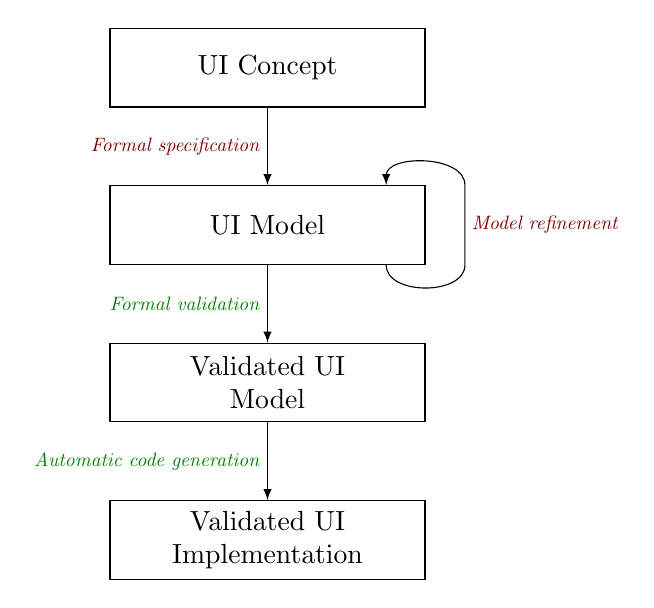
\begin{tikzpicture}

\node[processstep] (S1) at (0cm,6cm) {UI Concept};
\node[processstep] (S2) at (0cm,4cm) {UI Model};
\node[processstep] (S3) at (0cm,2cm) {Validated UI \\ Model};
\node[processstep] (S4) at (0cm,0cm) {Validated UI \\ Implementation};

\coordinate[justright] (S2NORTHEAST1) at (S2.north east);
\coordinate[justright] (S2SOUTHEAST1) at (S2.south east);
\coordinate[justleft] (S2NORTHEAST2) at (S2.north east);
\coordinate[justleft] (S2SOUTHEAST2) at (S2.south east);

\draw[orientedarc] (S1) -- (S2) node[arclabelred, left]{\textit{Formal specification}};
\draw[orientedarc] (S2) -- (S3) node[arclabelgreen, left]{\textit{Formal validation}};
\draw[orientedarc] (S3) -- (S4) node[arclabelgreen, left]{\textit{Automatic code generation}};
\draw[orientedarc] (S2SOUTHEAST2) to[bend right=90] (S2SOUTHEAST1) -- (S2NORTHEAST1) node[arclabelred, right]{\textit{Model refinement}} to[bend right=90] (S2NORTHEAST2);

\end{tikzpicture}
}

\caption{Proposed UI conception process}
\label{fig:process3}
\end{figure}

New tools have been developed in order to enhance this heavy process. Some of these tools can be used in order to generate an abstract model of the UI, taking its code as an input, allowing to perform formal validation on the implemented UI \cite{Cortier2008}. Other methods allow to specify UIs using specific languages in order to validate critical parts \cite{madani2007}.

However, a common language allowing an efficient collaboration of these different tools does not exist yet. That is why critical UIs development process can become complex and costly (see Fig~\ref{fig:process2}). 

Progress toward a straightforward conception process (see Fig~\ref{fig:process3}) is required to the conception of future UIs. The existence of a formal language taking into account all the aspects of critical UIs (see Fig~\ref{fig:domains}) would greatly help to fulfil this goal.


%====================================================================================================================================
% SECTION
%====================================================================================================================================
\section{APPLICATIONS}% What are the application domains where the approach has been applied?
The application field of this formal language will be formal specification, verification and validation of ARINC 661 compliant UAs.

By enhancing the development process, this approach aims at reducing development costs of critical UIs. 
The approach could allow to shorten testing phases and to reduce development cycles time.

%====================================================================================================================================
% SECTION
%====================================================================================================================================
\section{LIMITATIONS AND DEVELOPMENT OPPORTUNITIES}% What are the known limitations/development opportunities for the framework?

The language will be limited to embedded critical UIs complying with the ARINC 661 specification. Thus, the following limitations will exist:
\begin{packed_itemize}
\item{Graphical user interfaces only} 
\item{No dynamic instantiation of widgets (UI structure specified at conception time, no modifications at run time)}
\item{No concern about rendering and  other low level concerns (Dealt with the CDS, outside of our scope)}
\end{packed_itemize}

In a first approach, we will target the work around modelling the complexity of UI dynamic behaviour, dropping the following concerns:
\begin{packed_itemize}
\item{Look\&Feel (formatting, colouring, screen structure)} 
\item{Human factors (usability analysis, ergonomics)}
\end{packed_itemize}

However, the language will be designed to be as expandable as possible, in order to ease future developments.

% Balancing columns in a ref list is a bit of a pain because you
% either use a hack like flushend or balance, or manually insert
% a column break.  http://www.tex.ac.uk/cgi-bin/texfaq2html?label=balance
% multicols doesn't work because we're already in two-column mode,
% and flushend isn't awesome, so I choose balance.  See this
% for more info: http://cs.brown.edu/system/software/latex/doc/balance.pdf
%
% Note that in a perfect world balance wants to be in the first
% column of the last page.
%
% If balance doesn't work for you, you can remove that and
% hard-code a column break into the bbl file right before you
% submit:
%
% http://stackoverflow.com/questions/2149854/how-to-manually-equalize-columns-in-an-ieee-paper-if-using-bibtex
%
% Or, just remove \balance and give up on balancing the last page.
%
\balance

% If you want to use smaller typesetting for the reference list,
% uncomment the following line:
% \small
\bibliographystyle{acm-sigchi}
\bibliography{These}
\end{document}
